%!TEX root = volumeFinal.tex 

\chapter{\label{chap:ativ}Resultados - Avaliação de Desempenho}

Foram utilizados três mapas para avaliar o desempenho do algoritmo.
A avaliação dos resultados está divida por mapa.
Em cada mapa é possível jogar em dois lados.
O lado azul começa o jogo na parte superior do mapa, e o lado vermelho começa na parte inferior.
Em cada mapa é avaliado a porcentagem de vitórias para cada domínio.
Os adversários, utilizados para testar o algoritmo, são as técnicas presentes no MicroRTS apresentadas na Seção~\ref{sec:tecn}.
Cada adversário foi utilizado dez vezes em cada mapa, e em cada lado do jogo.

\section{Mapa 1}


O mapa 1 tem o tamanho de 16 por 16
Os experimentos foram executados em um mapa 16 por 16 e com o algoritmo começando dos dois lados do jogo, o lado azul na parte superior, e o lado vermelho na parte inferior. Cada jogador inicia possuindo uma base, um trabalhador e dois recursos próximos a sua base.


descreve o mapa.

\begin{figure}[ht]
	\centering
	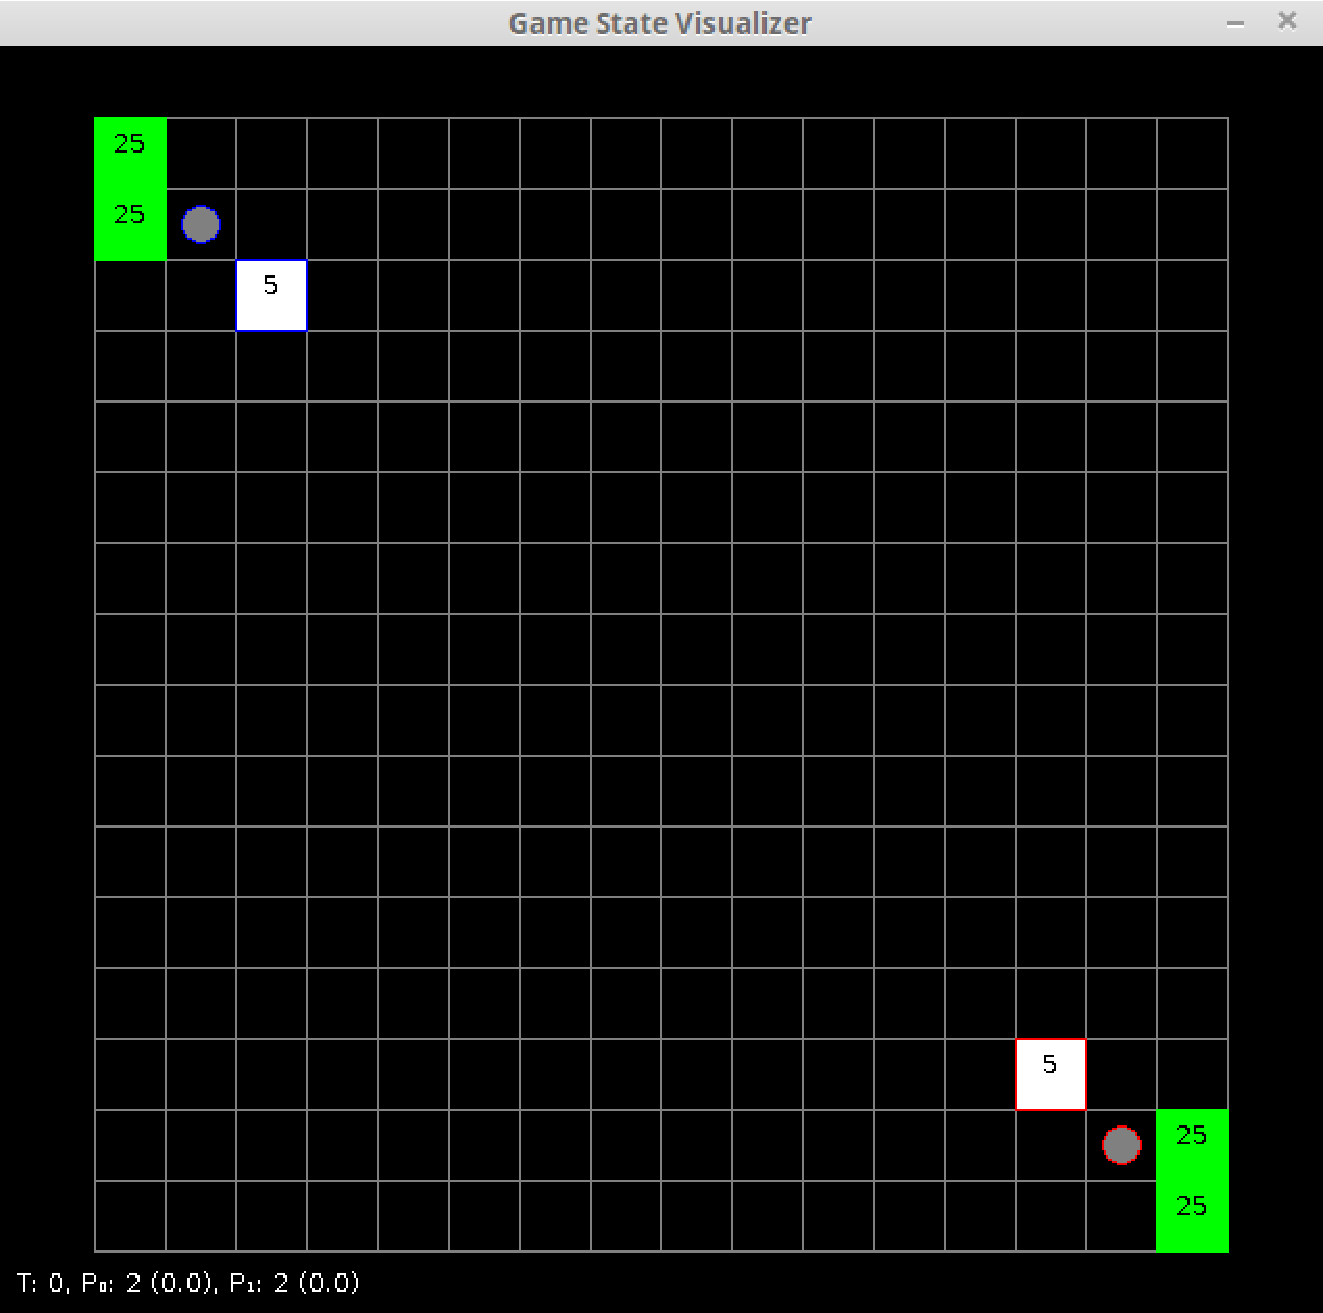
\includegraphics[width=.6\textwidth]{fig/map16x16.pdf}
	\caption{Configuração inicial do mapa 1.}
	\label{fig:mapa16x16}
\end{figure}


explica a tabela


\begin{table}[ht]
	\centering
	\caption{Porcentagem de vitórias no mapa 1.}
	\label{tab:mapa1}
	\begin{tabular}{|c|cc|cc|}
		\hline
		\textbf{}           & \multicolumn{2}{c|}{\textbf{Estratégia 1}}  & \multicolumn{2}{c|}{\textbf{Estratégia 2}}  \\ \hline
		\textbf{Adversário} & \textbf{Lado Azul} & \textbf{Lado Vermelho} & \textbf{Lado Azul} & \textbf{Lado Vermelho} \\ \hline
		RandomIA            & 100\%              & 100\%                  & 100\%              & 100\%                  \\ \hline
		RandomBiasedIA      & 80\%               & 100\%                  & 100\%              & 100\%                  \\ \hline
		RangedRush          & 0\%                & 100\%                  & 100\%              & 100\%                  \\ \hline
		HeavyRush           & 0\%                & 100\%                  & 0\%                & 100\%                  \\ \hline
		LightRush           & 0\%                & 100\%                  & 0\%                & 100\%                  \\ \hline
		WorkerRush          & 0\%                & 0\%                    & 0\%                & 0\%                    \\ \hline
		MonteCarlo          & 60\%               & 80\%                   & 100\%              & 100\%                  \\ \hline
		Minimax             & 100\%              & 100\%                  & 100\%              & 100\%                  \\ \hline
		Portfolio           & 0\%                & 0\%                    & 0\%                & 0\%                    \\ \hline
	\end{tabular}
\end{table}

conclui alguma coisa

\section{Mapa 2}


\begin{figure}[ht]
	\centering
	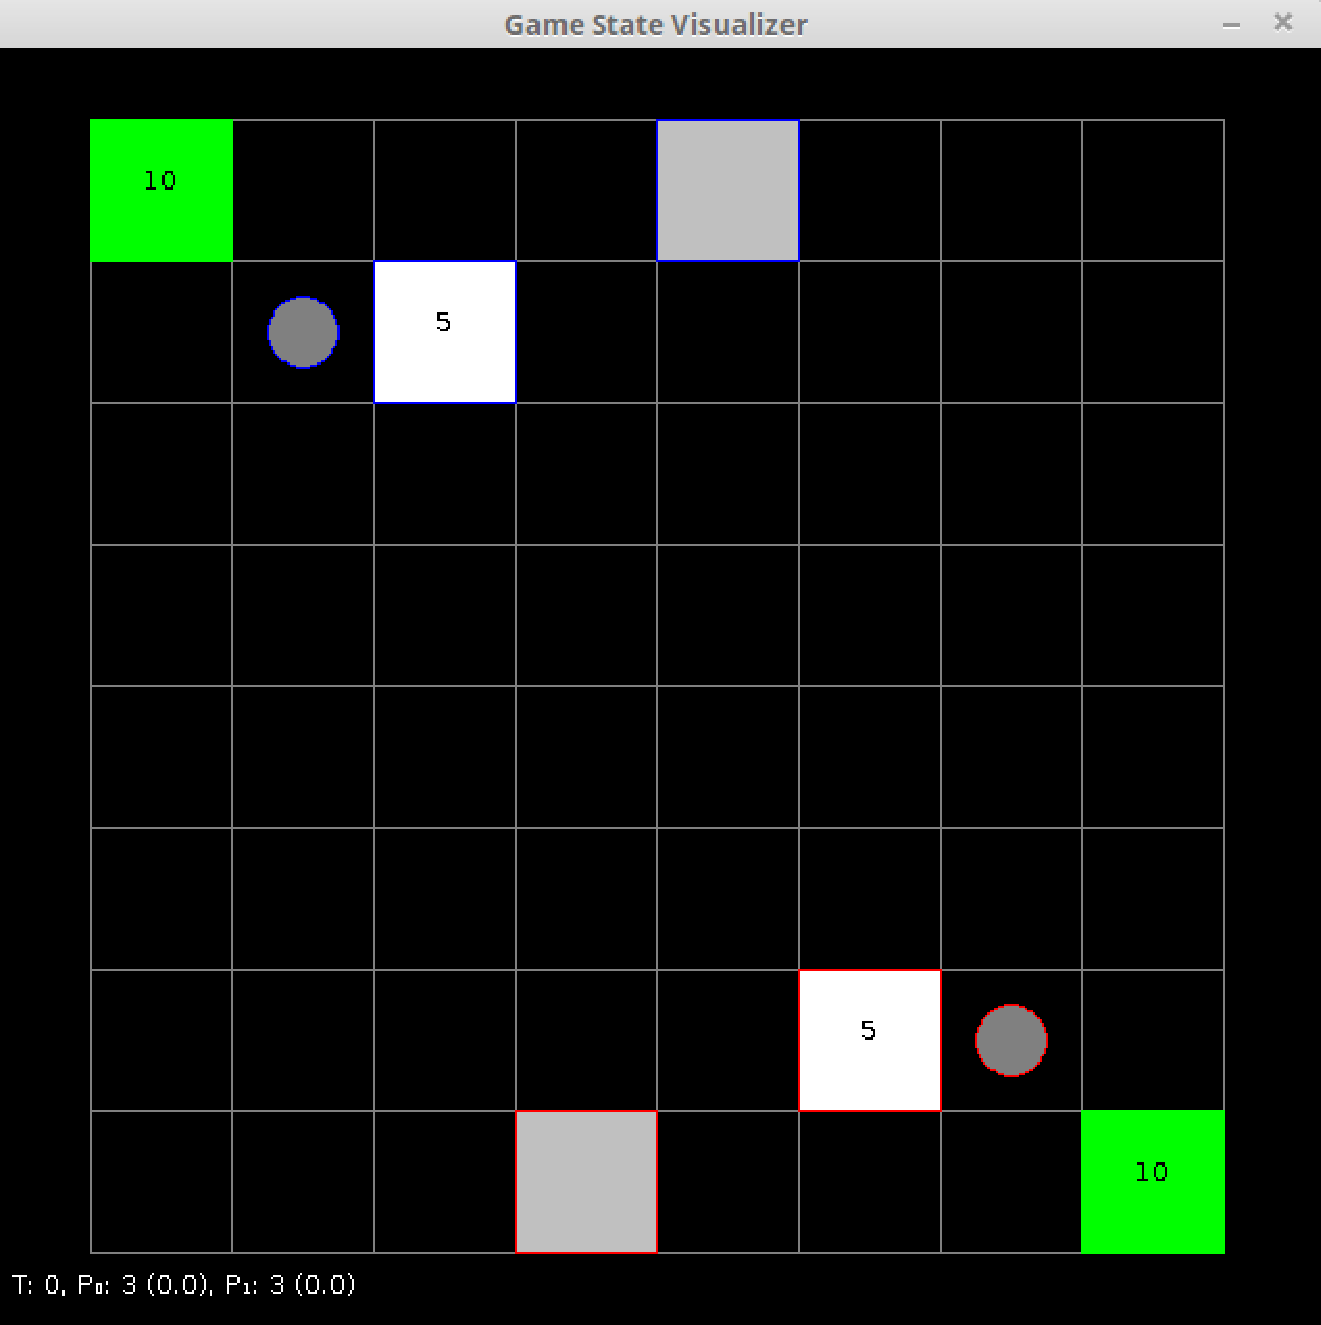
\includegraphics[width=.6\textwidth]{fig/map8x8quartel.pdf}
	\caption{Configuração inicial do mapa 2.}
	\label{fig:mapa8x8quartel}
\end{figure}

\begin{table}[ht]
	\centering
	\caption{Porcentagem de vitórias no mapa 2.}
	\label{tab:mapa2}
	\begin{tabular}{|c|cc|cc|}
		\hline
		\textbf{}           & \multicolumn{2}{c|}{\textbf{Estratégia 1}}  & \multicolumn{2}{c|}{\textbf{Estratégia 2}}  \\ \hline
		\textbf{Adversário} & \textbf{Lado Azul} & \textbf{Lado Vermelho} & \textbf{Lado Azul} & \textbf{Lado Vermelho} \\ \hline
		RandomIA            & 100\%              & 100\%                  & 100\%              & 100\%                  \\ \hline
		RandomBiasedIA      & 40\%               & 80\%                   & 80\%               & 100\%                  \\ \hline
		RangedRush          & 0\%                & 100\%                  & 0\%                & 100\%                  \\ \hline
		HeavyRush           & 0\%                & 100\%                  & 0\%                & 100\%                  \\ \hline
		LightRush           & 0\%                & 100\%                  & 0\%                & 100\%                  \\ \hline
		WorkerRush          & 0\%                & 0\%                    & 0\%                & 0\%                    \\ \hline
		MonteCarlo          & 0\%                & 0\%                    & 0\%                & 0\%                    \\ \hline
		Minimax             & 0\%                & 100\%                  & 0\%                & 100\%                  \\ \hline
		Portfolio           & 0\%                & 100\%                  & 0\%                & 100\%                  \\ \hline
	\end{tabular}
\end{table}

\section{Mapa 3}

\begin{figure}[ht]
	\centering
	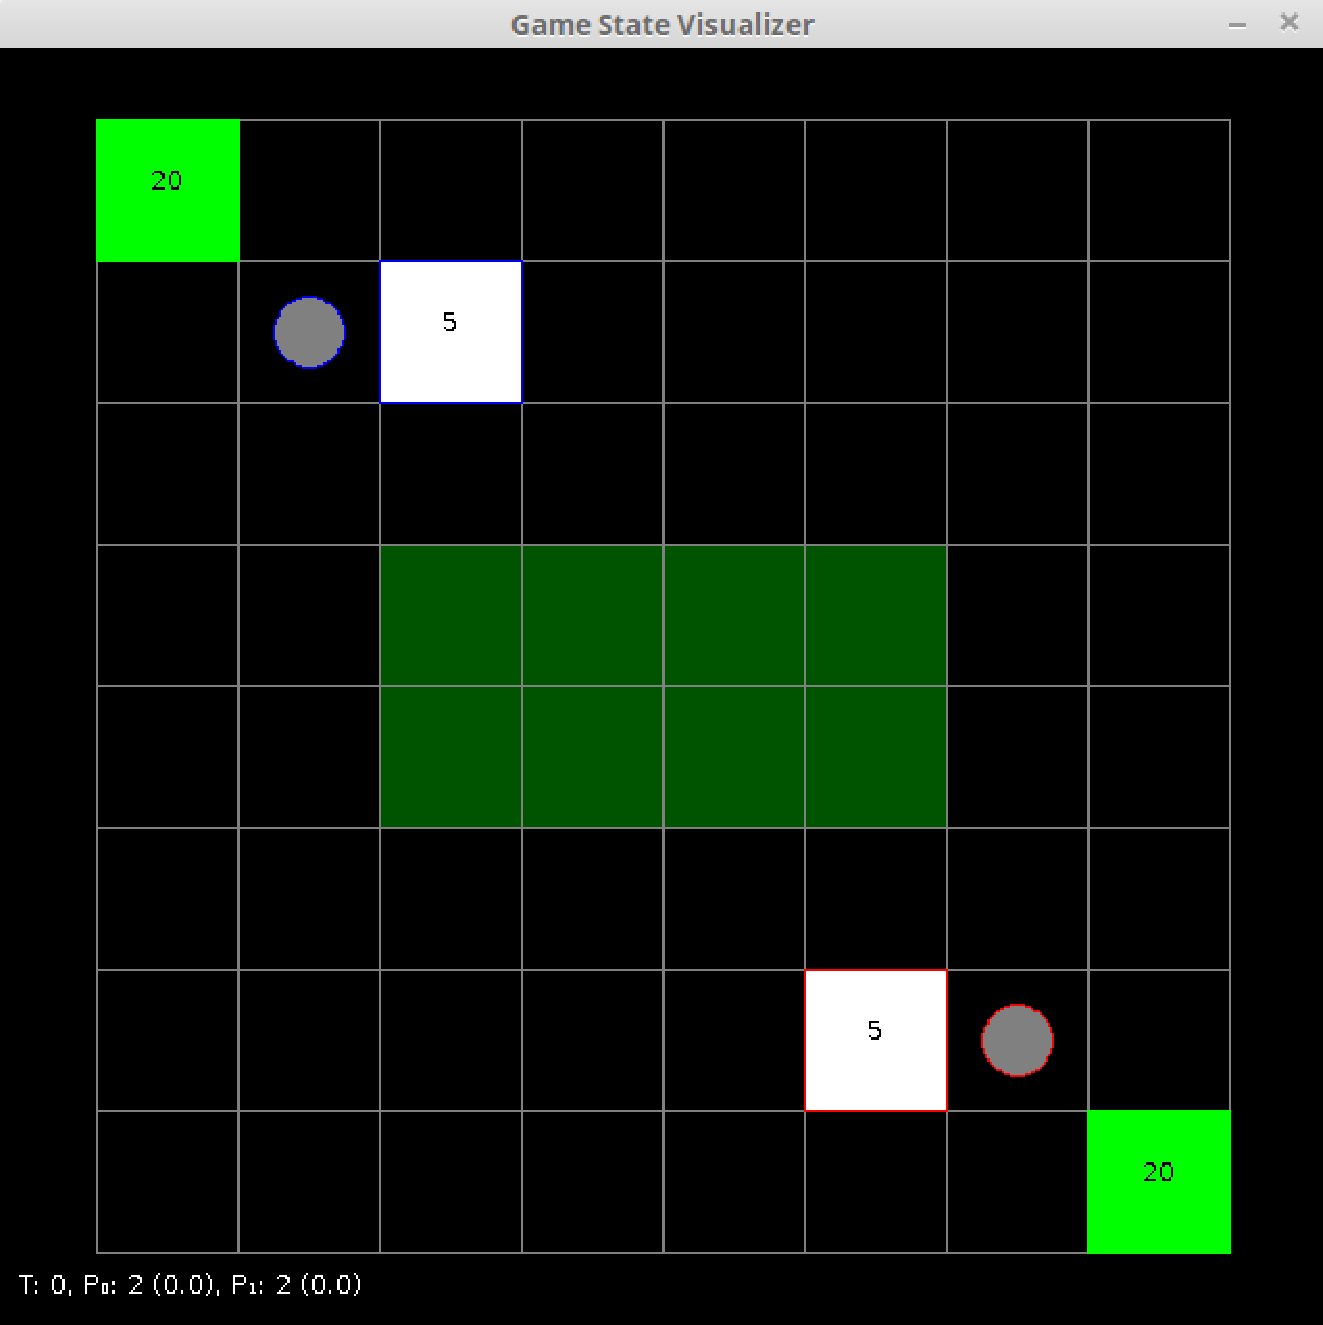
\includegraphics[width=.6\textwidth]{fig/map8x8obsta.pdf}
	\caption{Configuração inicial do mapa 3.}
	\label{fig:mapa8x8obsta}
\end{figure}

\begin{table}[ht]
	\centering
	\caption{Porcentagem de vitórias no mapa 3.}
	\label{tab:mapa3}
	\begin{tabular}{|c|cc|cc|}
		\hline
		\textbf{}           & \multicolumn{2}{c|}{\textbf{Estratégia 1}}  & \multicolumn{2}{c|}{\textbf{Estratégia 2}}  \\ \hline
		\textbf{Adversário} & \textbf{Lado Azul} & \textbf{Lado Vermelho} & \textbf{Lado Azul} & \textbf{Lado Vermelho} \\ \hline
		RandomIA            & 100\%              & 100\%                  & 100\%              & 100\%                  \\ \hline
		RandomBiasedIA      & 100\%              & 80\%                   & 100\%              & 80\%                   \\ \hline
		RangedRush          & 0\%                & 100\%                  & 0\%                & 100\%                  \\ \hline
		HeavyRush           & 0\%                & 100\%                  & 0\%                & 100\%                  \\ \hline
		LightRush           & 0\%                & 100\%                  & 0\%                & 100\%                  \\ \hline
		WorkerRush          & 0\%                & 0\%                    & 0\%                & 0\%                    \\ \hline
		MonteCarlo          & 0\%                & 0\%                    & 0\%                & 0\%                    \\ \hline
		Minimax             & 0\%                & 100\%                  & 100\%              & 80\%                   \\ \hline
		Portfolio           & 0\%                & 0\%                    & 0\%                & 0\%                    \\ \hline
	\end{tabular}
\end{table}


\section{Tamanho de cada IA}

\begin{table}[ht]
	\centering
	\caption{Tamanho  do código de cada técnica.}
	\label{tab:tamanho}
	\begin{tabular}{|c|c|}
		\hline
		\textbf{Adversário} & \textbf{Tamanho} \\ \hline
		Domínio 1           & 11,3 kB          \\ \hline
		Domínio 2           & 11,5 kB          \\ \hline
		RandomIA            & 4,0 kB           \\ \hline
		RandomBiasedIA      & 4,6 kB           \\ \hline
		RangedRush          & 13,7 kB          \\ \hline
		HeavyRush           & 14,0 kB          \\ \hline
		LightRush           & 14,0 kB          \\ \hline
		WorkerRush          & 13,6 kB          \\ \hline
		MonteCarlo          & 18,1 kB          \\ \hline
		Minimax             & 12,9 kB          \\ \hline
		Portfolio           & 14,4 kB          \\ \hline
	\end{tabular}
\end{table}

\section{tempo de geração das ações do algoritmo}

Mostrar o tempo de gerar as ações que é alto no inicio e baixo no final
colocar gráficos aqui 


tempo para gerar as ações
da pra fazer uma tabela aqui com o tempo de cada técnica



\begin{itemize}
	\item BenchMark
	\item explicação dos resultados
	\item porcentagem de vitorias
	\item tempo de gerar cada ação
	\item tamanho de cada IA	
\end{itemize}

